\documentclass[12pt,a4,english,finnish,pdflatex%,handout
]{beamer}
\definecolor{MyGreen}{RGB}{50, 120, 50}
\usecolortheme[named=MyGreen]{structure}

\usepackage{babel}
\usepackage[utf8]{inputenc}
\usepackage[T1]{fontenc}
\usepackage{amsmath,amssymb} 
\usepackage{animate}
\usepackage{multimedia}

\usepackage{natbib}
\bibpunct[: ]{(}{)}{,}{}{}{;}

\usepackage{tikz}

\usepackage{tipa}

\usepackage{hyperref}

\setbeamertemplate{navigation symbols}{}

\graphicspath{{figures/}}

\setlength{\leftmargini}{0pt}
\setlength{\leftmarginii}{1em}

\newcommand{\kommentti}[1]{
  {\bf[#1]}
}



\begin{document}
\title{Kieliultraäänidatan analyysimenetelmiä\\
  a.k.a. UltraLuento 2.
} 
\author{Pertti Palo} \date{28. maaliskuuta 2021}

\frame{\titlepage
} 

\frame{\frametitle{Edellisen kerran sisältöä}
  \begin{itemize}
  \item 1. Luento: Ultraäänikuvauksen ominaisuudet toimintaperiaate
    \begin{itemize}
    \item Etuja
    \item Epäidaalisuuksia (eli puutteita)
    \item Fyysinen toimintaperiaate
    \end{itemize}
  \item 1. Luento: Puheartikulaation mittaaminen ultraäänellä
    \begin{itemize}
    \item Miltä kuva näyttää?
    \end{itemize}
  \end{itemize}

  \vfill
  \bf \Large 
  \usebeamercolor[fg]{title}
  Onko uusia tai vanhoja kysymyksiä?
}

\frame{\frametitle{2. UltraLuento: Ultraäänellä tallennetun puhemateriaalin analyysi}
  \begin{itemize}
  \item Osa I: Analyysimenetelmiä
    \begin{itemize}
    \item Audio -- siis tavallinen ääni
    \item Artikulatorinen data
      \begin{itemize}
      \item Kieliultraääni
      \item Kurkunpään ultraääni
      \item Huulivideot
      \end{itemize}
    \item Splinit: Tuottaminen ja analyysi
    \item Laskennalliset metriikat
    \end{itemize}
  \item Osa II: Data- ja analyysiesimerkkejä
  \end{itemize}
}

\frame{\frametitle{Audio}
  \begin{itemize}
  \item Tärkeä osa dataa on ultraäänen kanssa yhdessä synkronoidusti
    tallennettu ääni.
  \item Ääntä voi analysoida AAA-ohjelmassa, mutta se on helpompaa
    Praat-ohjelmalla.
  \item Akustisen segmentoinnin tuloksista on huomattavaa hyötyä
    aineiston rajaamisessa. Niiden avulla artikulatorinen analyysi
    voidaan kohdistaa vain niihin ruutuihin, joista ollaan
    kiinnostuneita.
  \end{itemize}
}

\frame{\frametitle{Artikulatorinen data}
  \begin{itemize}
  \item Keskitymme tällä kertaa kieliultraäänen analyysiin.
  \item On kuitenkin hyvä huomata, että myös muita datatyyppejä tai
    -modaliteetteja voidaan yleensä tallentaa samalla laitteistolla --
    pienillä tai suurilla muutoksilla:
    \begin{itemize}
    \item Kurkunpään ultraääni käyttää yleensä erityyppistä anturia,
      joka pitää ostaa erikseen. Datan analyysi on tyypillisesti hyvin
      erilaista kuin kieliultraäänen analyysi, koska rakenteet ovat
      paljon monimutkaisempia.
    \item Huulivideoita voidaan tallentaa helposti. HY:n laitteistolla
      niitä saadaan joko kasvojen sivulta tai edestä. Huulivideoiden
      analyysiin on myös olemassa työkaluja.
    \item Suurempaa työtä vaatii yhtäaikainen datan tallennus
      esim. ultraäänellä ja elektromagneettisella artikulografialla
      tai muilla menetelmillä.
    \end{itemize}
  \end{itemize}
}

\frame{\frametitle{Pelkät videot tai kuvat}
  \begin{itemize}
  \item Ultraäänivideoita voidaan annotoida siinä missä mitä hyvänsä
    videoita.
  \item Työ ei ole ihan kevyttä, joten aiheen ja materiaalin
    rajauksessa kannattaa olla huolellinen.
  \item Annotoinnin voi tehdä AAA-ohjelmassa tai esimerkiksi
    .avi-formaatissa tallenettuja videoita voi käsitellä videoiden
    annotointiin tarkoitetuilla ohjelmilla.
  \item Yksittäisistä kuvista voi myös tehdä suoria mittauksia.
  \end{itemize}
}

\frame{\frametitle{Splinit I}
  \hspace*{-.5cm}
  \centering
  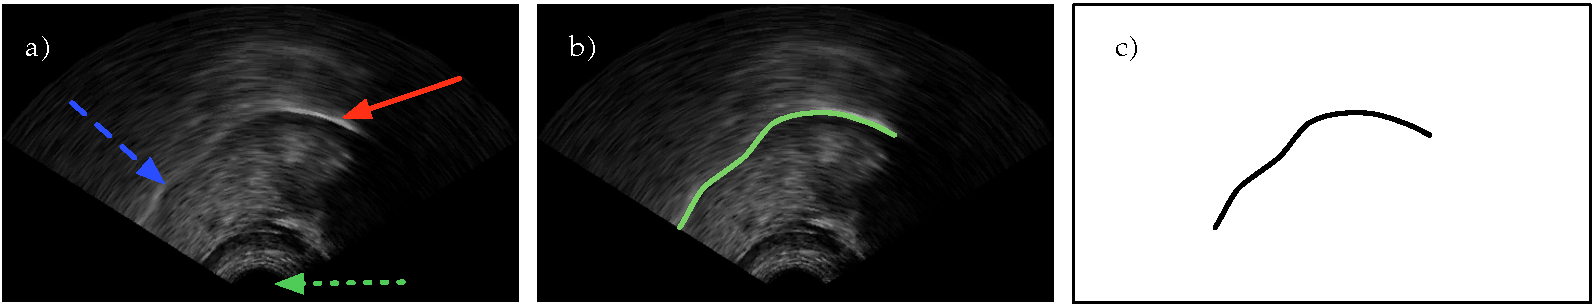
\includegraphics[width=1.05\textwidth]{P2_lemon_1st_frame_spline.pdf}
  \hspace*{.5cm}
  \begin{itemize}
  \item Splinin sovitus ultraäänikuvaan tarkoittaa, että piirrämme
    kielen pinnan mukaisen käyrän ultraäänikuvaan - tai oikeastaan
    asetamme splinin ohjauspisteet kuvaan.
  \item Sovitus voidaan tehdä joko manuaalisesti tai automaattisesti.
  \item Automaattista tulosta voidaan myös korjata manuaalisesti.
  \end{itemize}
}

\frame{\frametitle{Splinit II}

\begin{itemize}
  \item Tulokset riippuvat paljon datan laadusta:
  \begin{itemize}
  \item Selkeisiin kuviin on helpompi sovittaa splini.
  \item Parempi paikkaresoluutio auttaa, mutta ei takaa, sovittamisen
    onnistumista.
  \end{itemize}
  \item Splinit itsessään voivat olla analyysin tulos ja niitä voidaan
  verrata toisiinsa silmämääräisesti.
  
\end{itemize}
}

\frame{\frametitle{Splinit III: Lähempi esimerkki}

\hspace*{-.5cm}
  \centering
  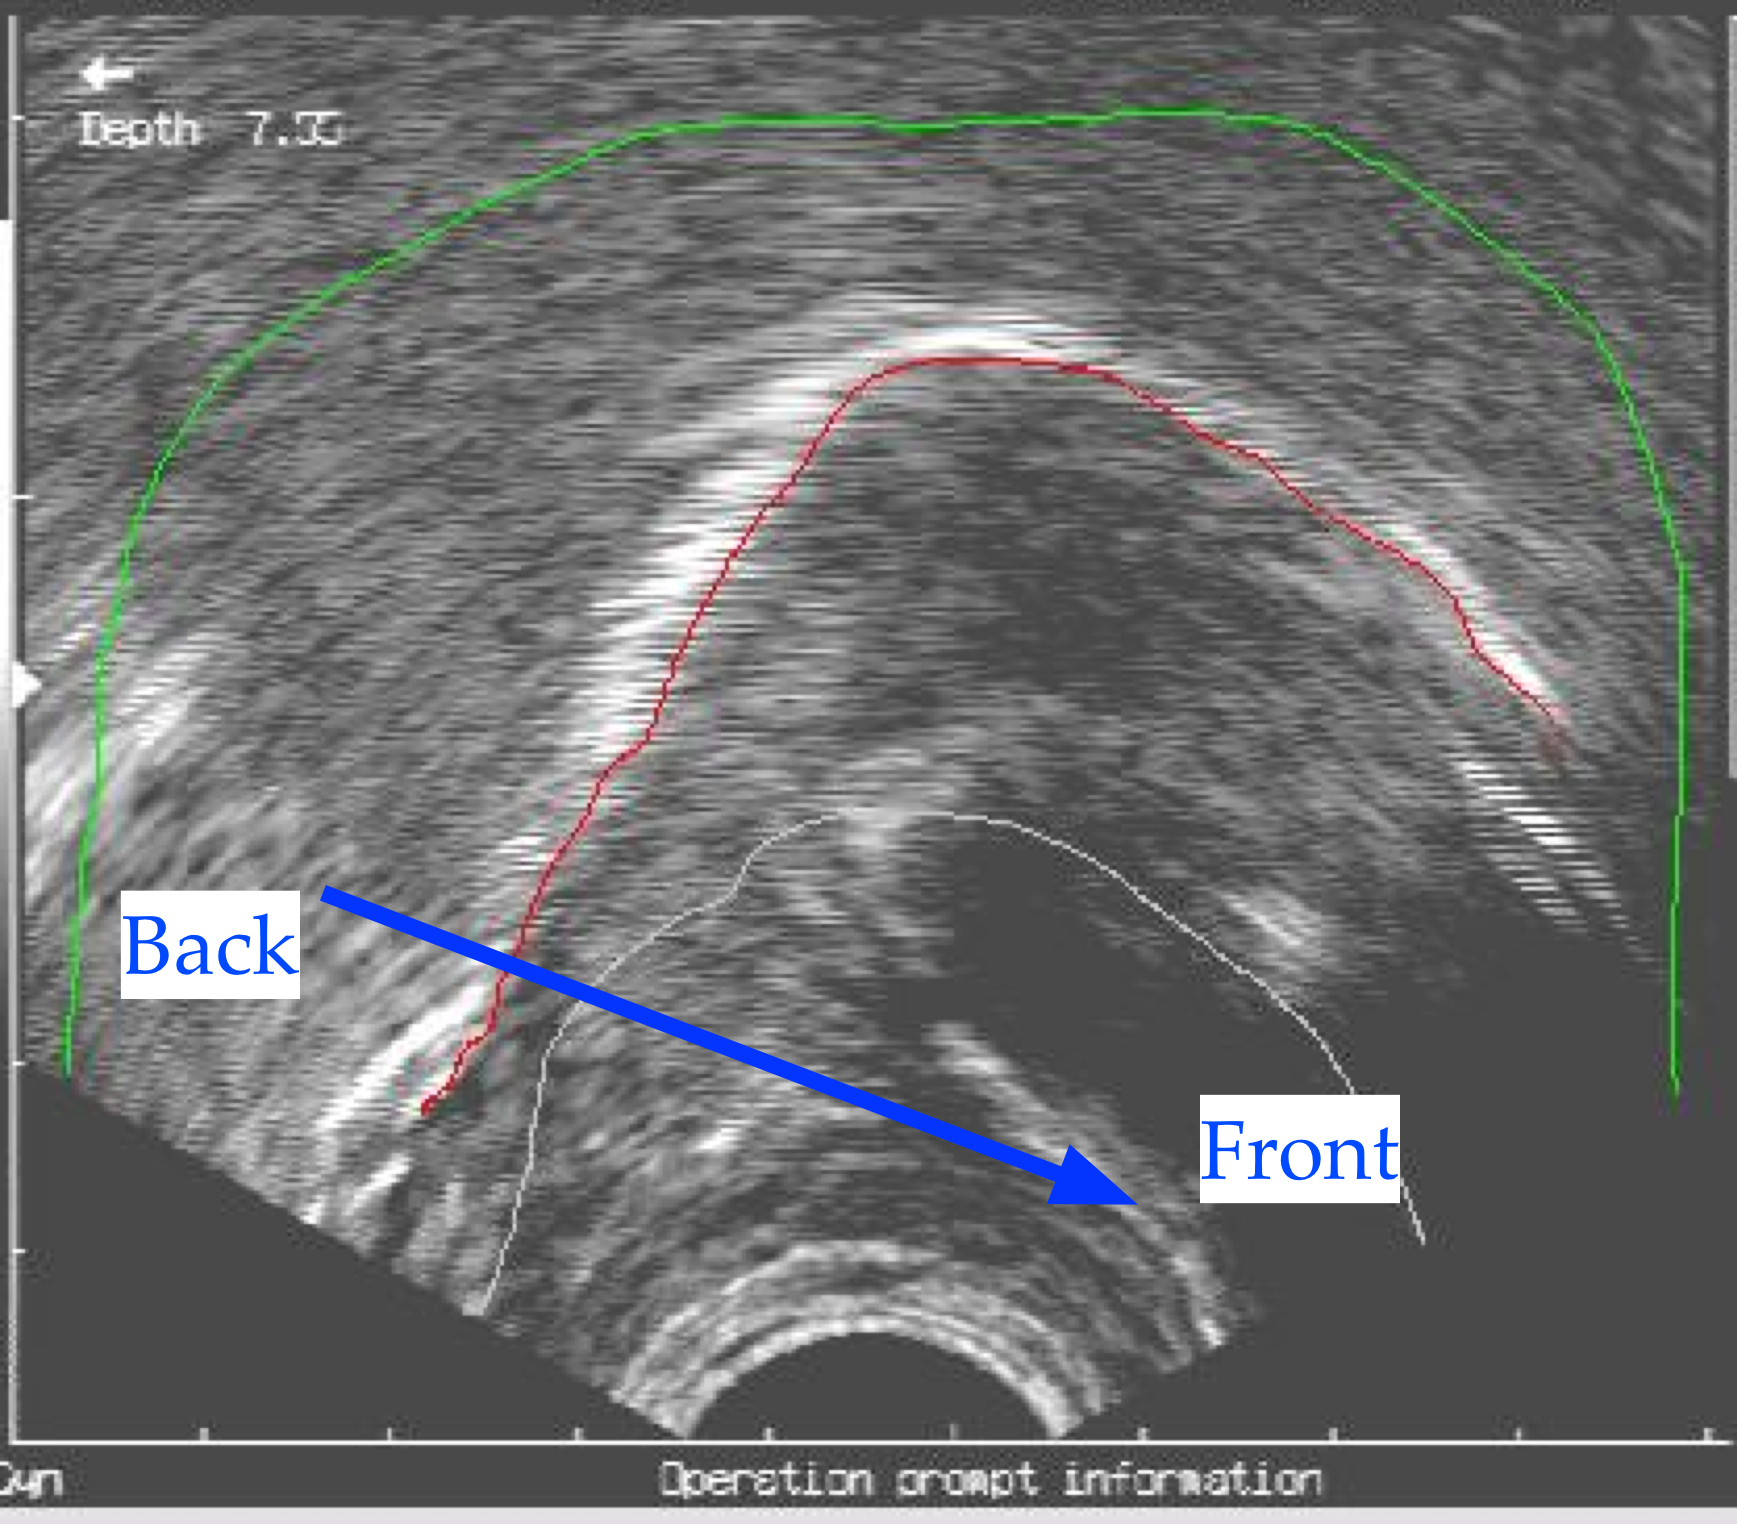
\includegraphics[width=.7\textwidth]{uti_traced}
}

\frame{\frametitle{Splinit IV: Analyysimenetelmiä}
  \hspace*{-.45cm}
  \centering
  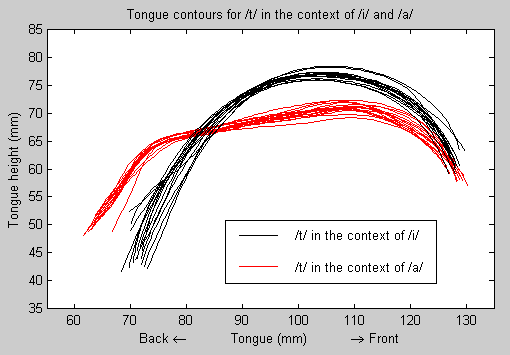
\includegraphics[width=.8\textwidth]{uti_contours}
  \vfill
  Perinteinen menetelmä: Valitaan audiosegmentaation perusteella
  ajasta kaksi tai useampia mielenkiintoisia pisteitä ja verrataan
  splinien muotoa niissä.
}
  
\frame{\frametitle{Splinit V: Analyysimenetelmiä}

  \hspace*{-.45cm}
  \centering
  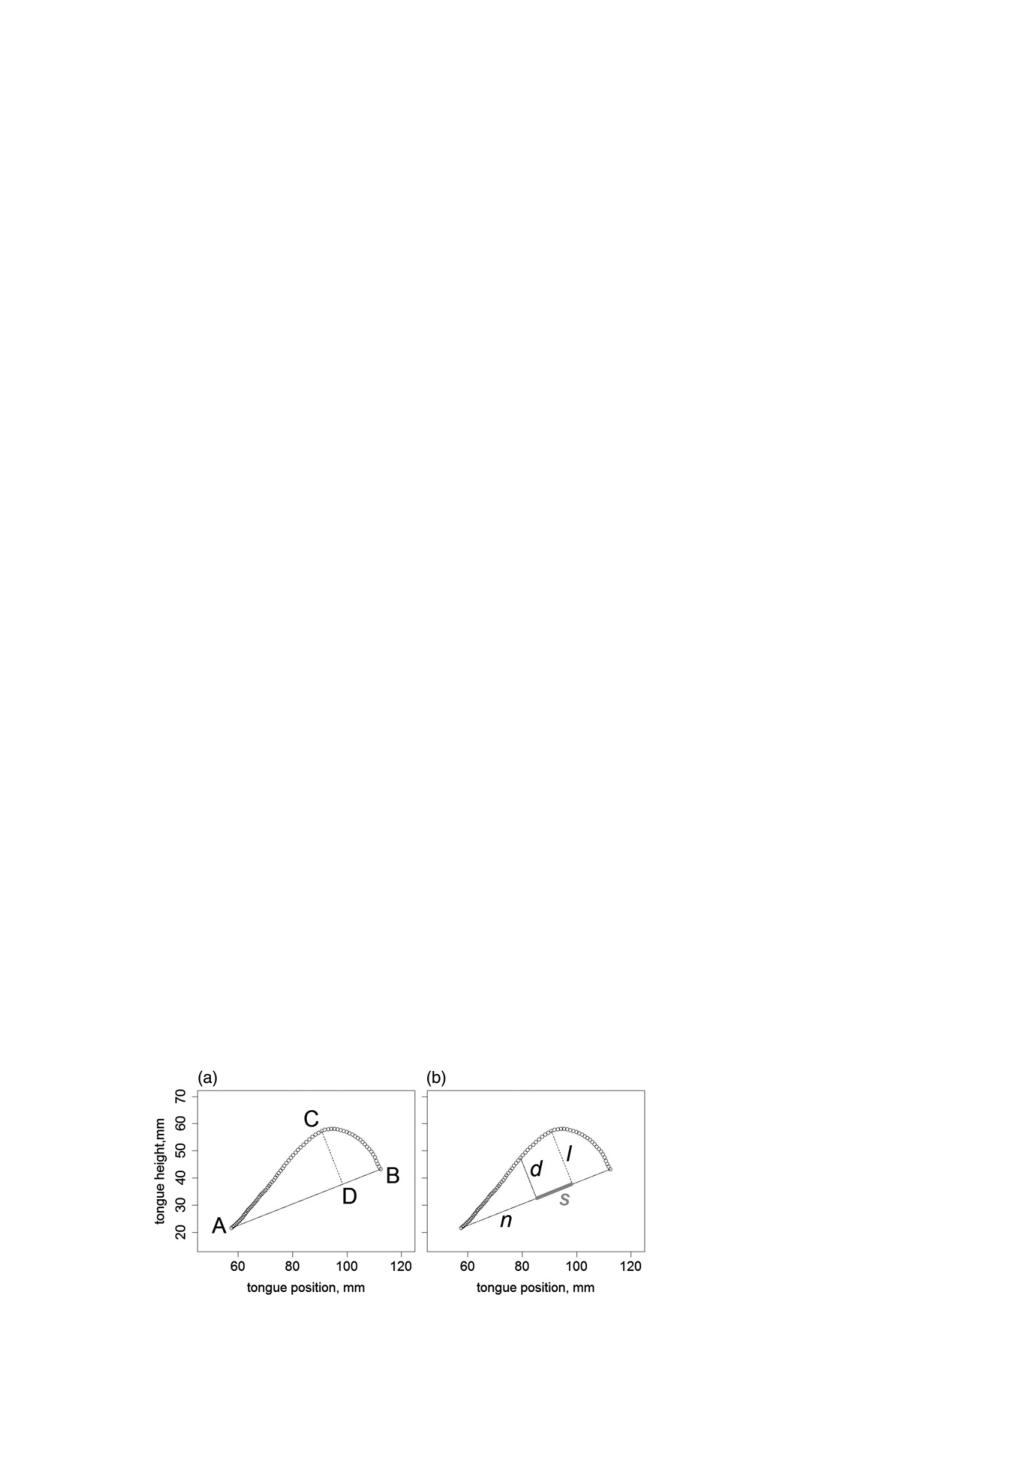
\includegraphics[width=.8\textwidth]{zharkova_metrics.pdf}

  \begin{itemize}
  \item Splinien muotoa voidaan analysoida myös ajan funktiona
    funktionaalisella data analyysilla ilman tarvetta rajoittua
    yksittäisiin ajanhetkiin analyysissä.
  \item Splineistä voidaan myös laskea erilaisia metriikoita ja
    verrata niitä sitä kautta toisiinsa. Esimerkiksi
    \cite{Zharkova:QLC:2015}.
  \item Menetelmiä on paljon ja erilaisiin kysymyksiin sopivat eri
    menetelmät.
  \end{itemize}
}

\frame{\frametitle{Laskennalliset metriikat}
  \begin{itemize}
  \item Voimme myös analysoida videoiden informaatiosisältöä
    erottamatta niistä kielenpintaa tai muita anatomisia
    rakenteita. Esimerkiksi:
    \begin{itemize}
    \item Pikselietäisyys (engl. Pixel Difference / PD, seuraavat
      kalvot) seuraa kokonaismuutosta ultraäänen raakadatan
      perusteella. Sopii erityisen hyvin liikkeen alun paikantamiseen.
    \item Optinen virta (engl. Optic flow) seuraa kuvan osien liikettä
      tilastollisin menetelmin ja arvioi mihin päin kuvan eri osat
      liikkuvat. Tämä on tärkeä menetelmä kurkunpään ultraäänen
      analyysissa.
    \item Kuvasarjojen suora tilastollinen analyysi
      \cite{Saito:USF:2020}.
    \end{itemize}
  \item Näitä ja muita menetelmiä voidaan käyttää myös splinien
    rinnalla tuomassa lisätietoa.
  \end{itemize}
}

\frame{
  \centering
  {
    \vfill
    \bf \Large 
    \usebeamercolor[fg]{title}
    Lyhyt tauko (5 min)
    \vfill
  }
}

\frame{
  \centering
  {
    \vfill
    \bf \Large 
    \usebeamercolor[fg]{title}
    Data- ja analyysiesimerkkejä
    \vfill
  }
}

\frame{\frametitle{Mitä dataa katsomme?}

  \begin{itemize}
  \item Tommi Nieminen \& Pertti Palo: Suomen \v{s}vaan artikulaatio.
    \begin{itemize}
    \item Aineistossa suomen lauseita epenteettisellä vokaalilla ja
      ilman.
    \item Pieni pilottiaineisto: Yksi epäluotettava puhuja.
    \item Hyvä aika- ja paikkaresoluutio, kuvat selkeitä.
    \end{itemize}
  \item Pertti Palo \& Sonja Dahlgren: Suomenkielen koartikulaatiotyypin pilotti.
    \begin{itemize}
    \item Aineistossa suomen sanoja ja epäsanoja.
    \item Julkaistavissa oleva pilottiaineisto: Kaksi luotettavaa puhujaa.
    \item Hyvä aika- ja paikkaresoluutio, kuvat kohtuullisen selkeitä.
    \end{itemize}
  \item Jalal Al-Tamimi \& Pertti Palo (forthcoming): ``Tongue
    contours in guttural consonants in Levantine Arabic: A Generalised
    Additive Modelling Approach''
    \begin{itemize}
    \item Aineistossa levantin arabinkielisiä sanoja.
    \item Laaja julkaisuihin tähtäävä aineisto: Puhujia kaikkiaan 10.
    \item Hyvä aikaresoluutio, paikkaresoluutio heikompi. Kuvat
      vähemmän selkeitä.
    \end{itemize}
  \end{itemize}
}

\frame{\frametitle{Analyysiesimerkki koartikulaatiodatasta}

  \begin{itemize}
  \item Segmentoidaan audio.
  \item Valitaan mielenkiintoiset kohdat.
  \item Splinitetään mielenkiintoiset kohdat.
  \item Korjataan splinit käsin.
  \item Lopuksi tehtäisiin AAA:ssa/R:ssä/Pythonilla splinianalyysia,
    mutta ei mennä niin pitkälle tänään.
  \end{itemize}
}


\frame{
  \centering
  {
    \vfill
    \bf \Large 
    \usebeamercolor[fg]{title}
    Kyselkää
    \vfill
  }
}


\frame{\frametitle{Kirjallisuutta ja kiitokset}
  \nocite{AlTamimi:TCG:2022,Dahlgren:SLS:2022}
  
  \begin{itemize}
  \item Steve Cowen: AAA:n käyttöapu ja kuva minusta.
  \item Felix Schaeffler: lepakkokuva.
  \item Alan Wrench: AAA:n käyttöapu ja laitteistokuvat.
  \end{itemize}
  
  \vspace*{.5cm}

  {\tiny
    \bibliographystyle{apalike}
    \bibliography{bib/master,bib/jpalo}
  }
}

\frame{\frametitle{Pikselietäisyys: Raakadata}
  \hspace*{-.5cm}
  \centering
  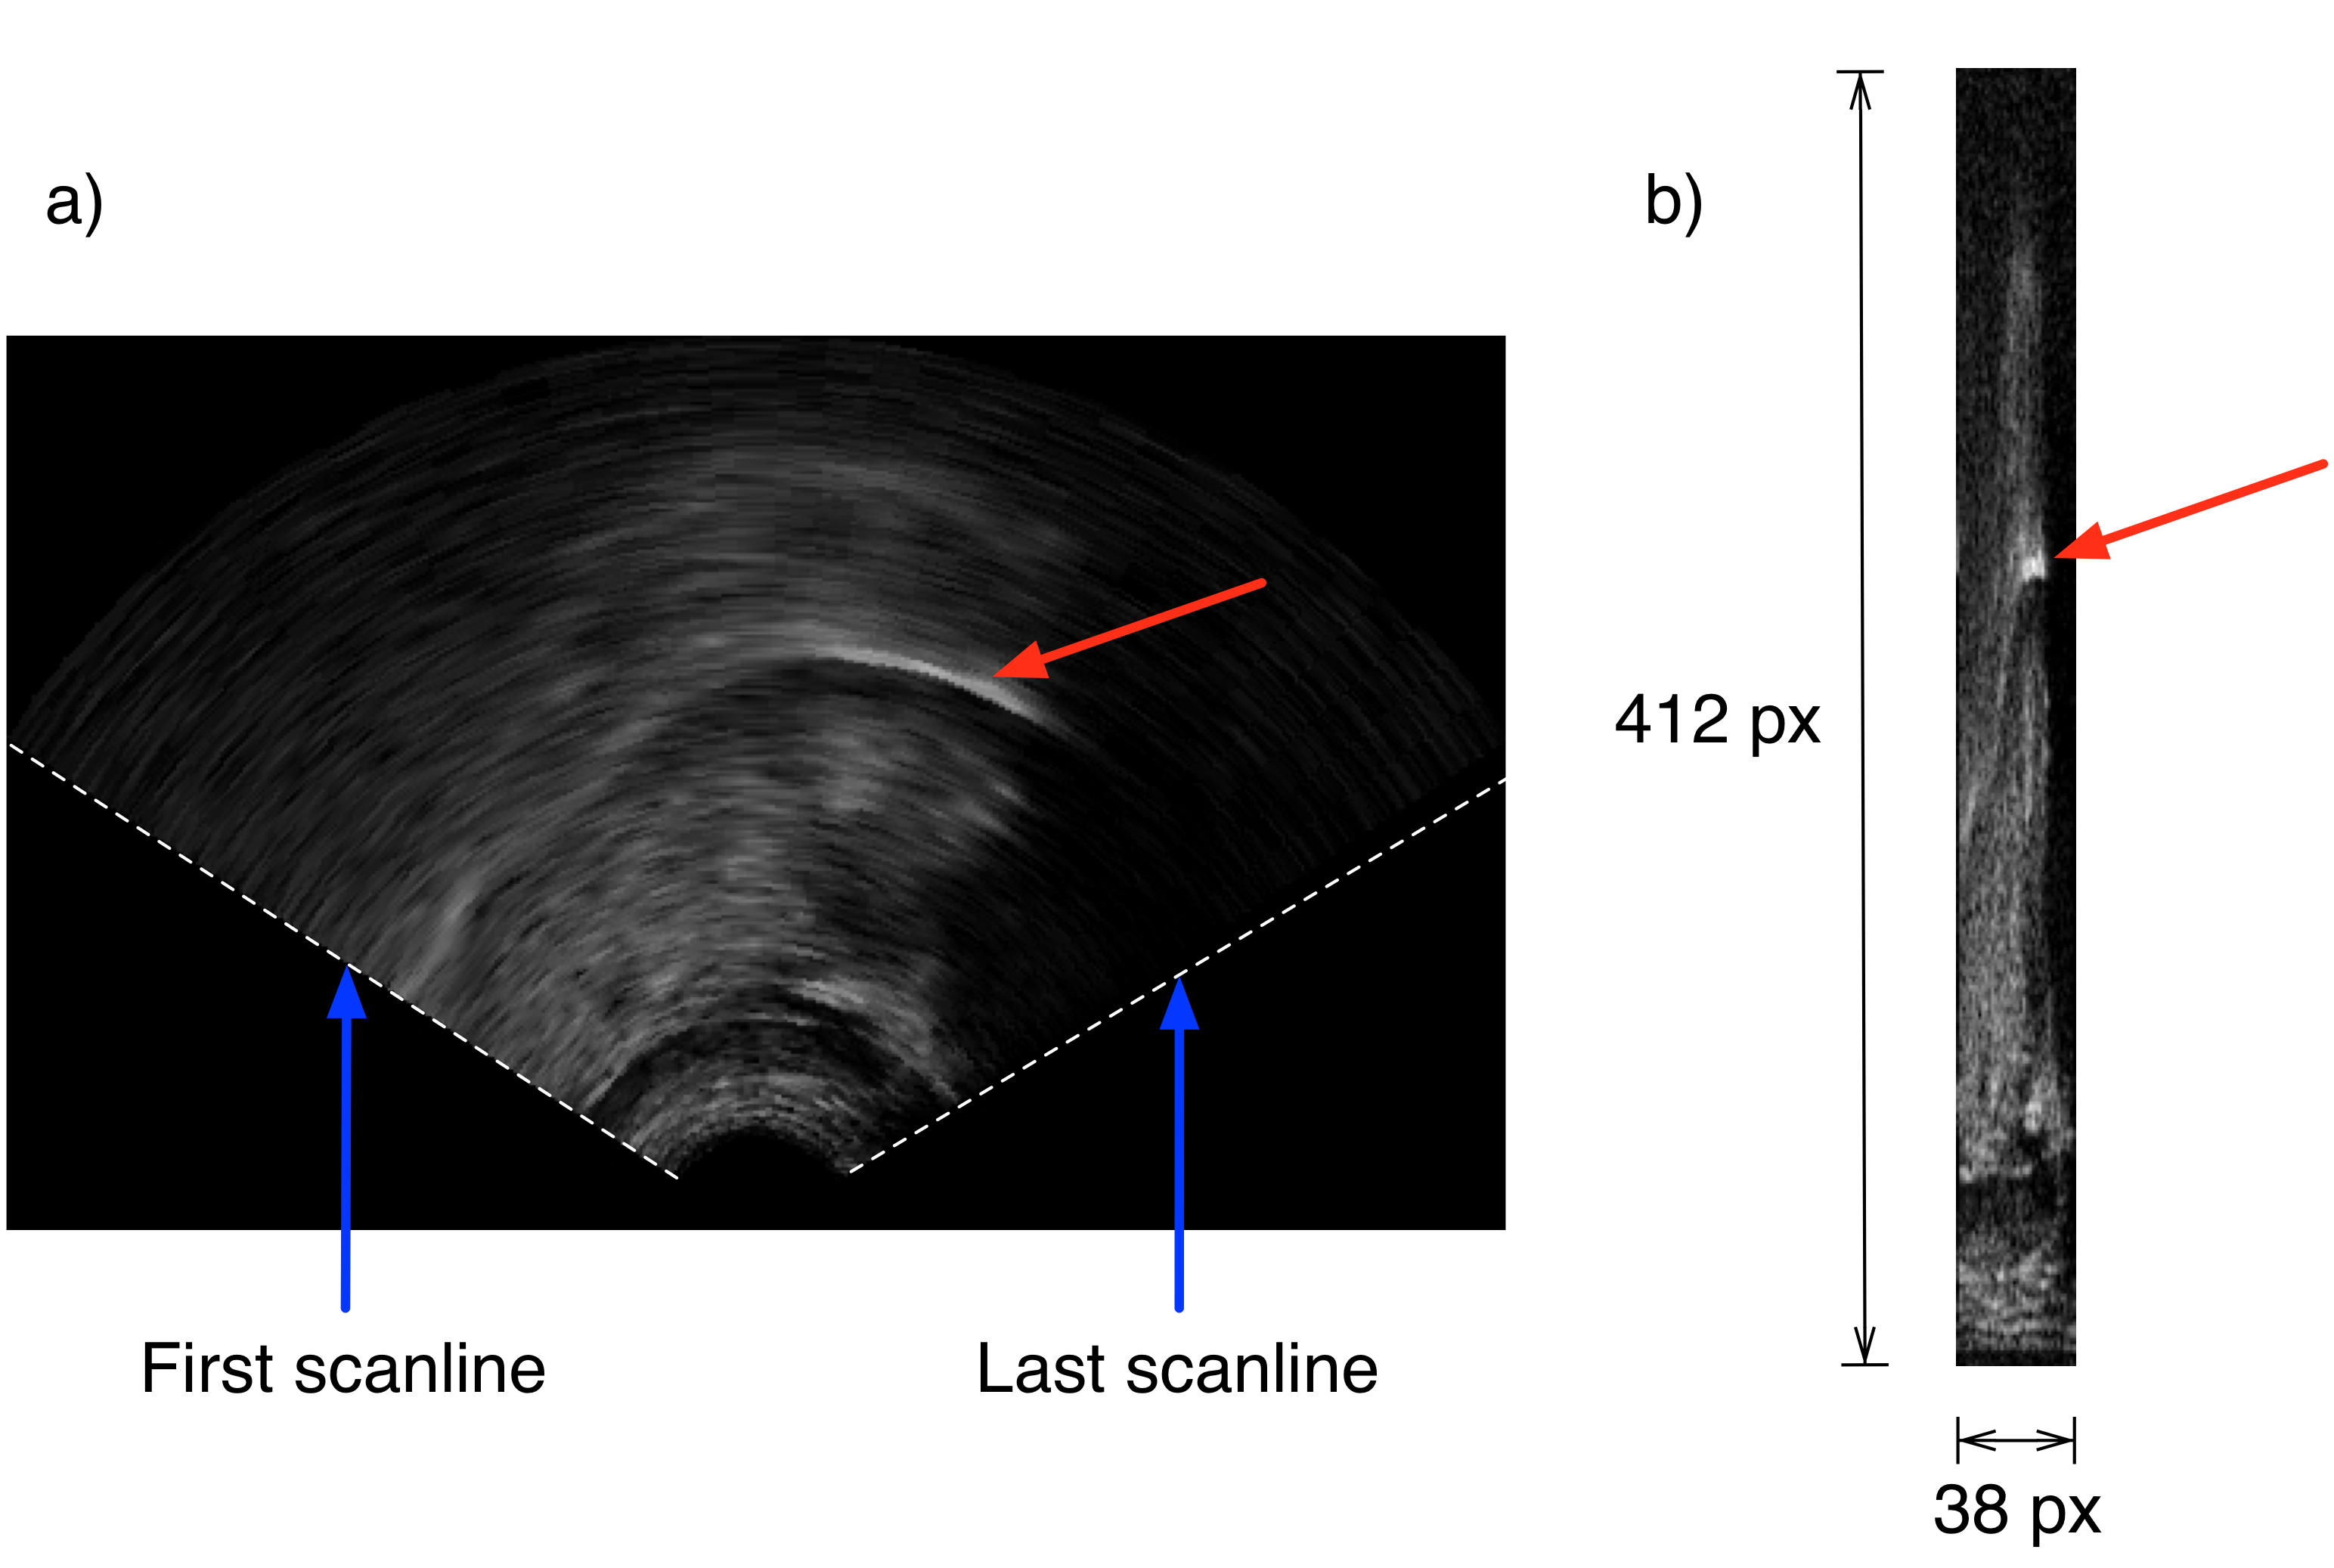
\includegraphics[width=1.05\textwidth]{P2_lemon_1st_frame_fan_v2.jpg}
}

\frame{\frametitle{Pikselietäisyys: Missä liike alkaa?}
  \hspace*{-.5cm}
  \centering
  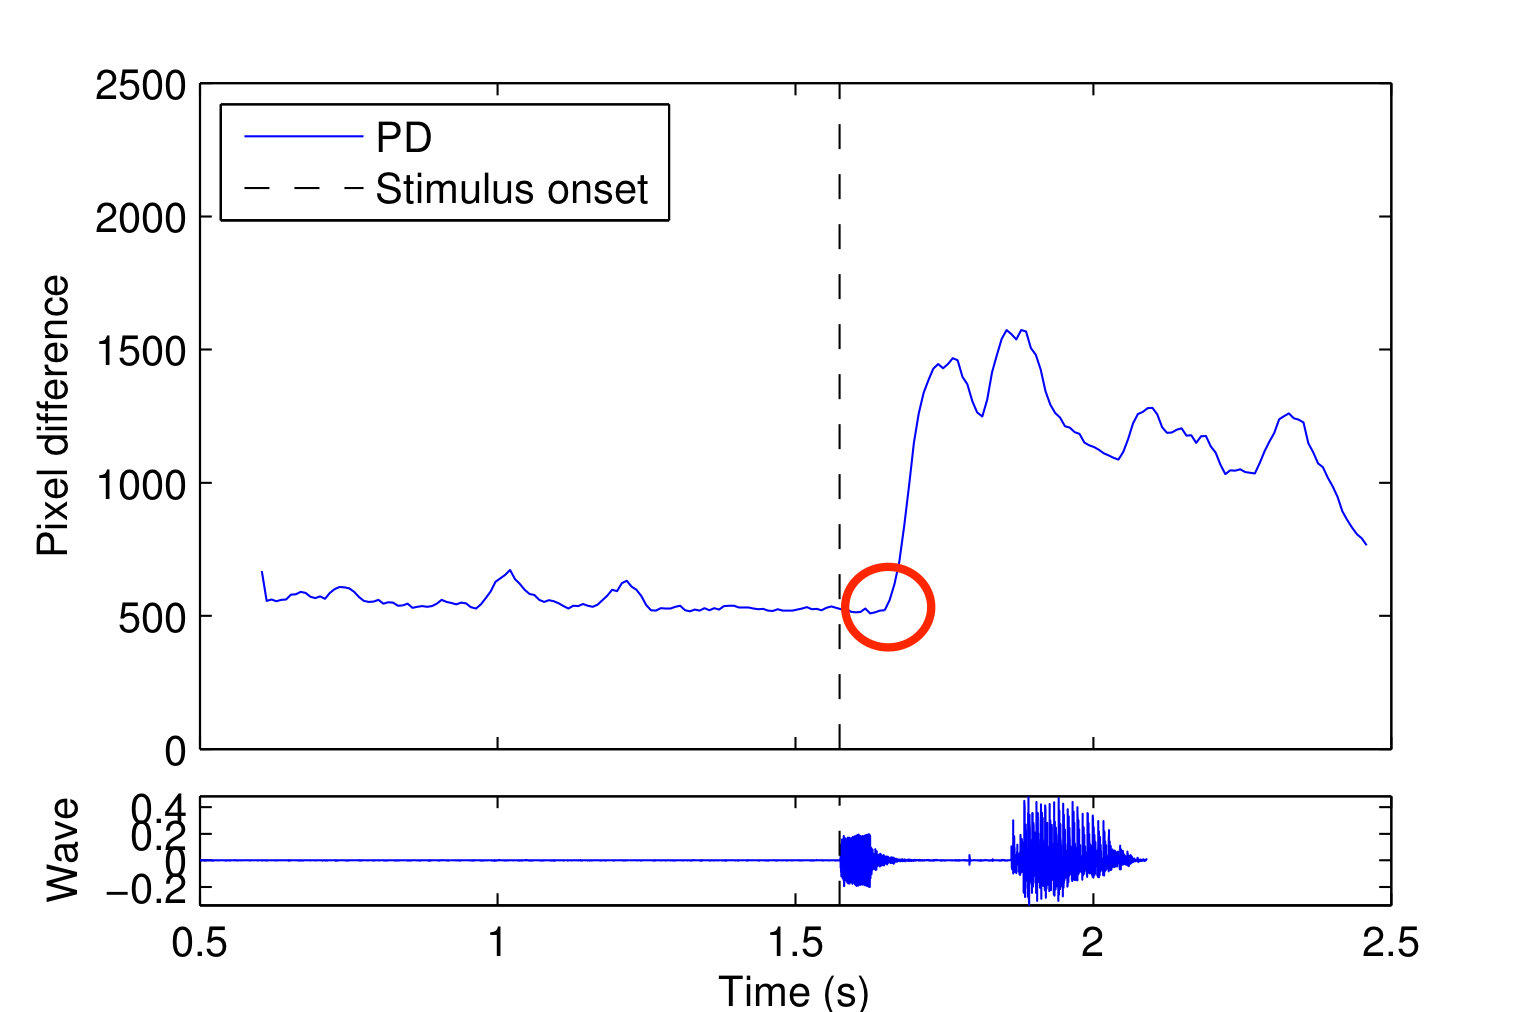
\includegraphics[width=\textwidth]{PD_annotated.jpg}
}

\end{document}

